\section{Dataset and Features}

%Give details about your dataset: how many training/validation/test examples do you have? What is the class label distribution of the dataset? Is there any preprocessing you did? What about normalization or data augmentation? What is the resolution of your images? If using video, how is it discretized?  Include a citation to where you got your dataset from.
%
%Depending on available space, show some examples from your dataset. You should also talk about the features you used. If you extracted features using Fourier transforms, word2vec, histogram of oriented gradients (HOG), PCA, ICA, etc. make sure to talk about it. Try to include examples of your data in the report (e.g. include an image, etc.).

We provide some details about our dataset below.

\subsection{Dataset Details}
For the milestone, we are using a dataset of food dishes collected from ImageNet~\cite{imagenet}. We plan to collect more images using the Bing Image Search API~\cite{bingimagesearchapi} in the future.

\subsection{Class Label Distribution}
Currently our dataset has 15 classes. Table~\ref{table:classdistribution} shows the class label distribution of the dataset. We do note that currently the distribution of images across the classes is not uniform. We plan to address this in the following weeks.

\subsection{Preprocessing Steps}

We re-sized all of our images to 32*32*3, by cropping the image if it was larger than the standard size, or adding black padding if it was smaller. We found that ImageNet~\cite{imagenet} tends to contain spurious images; it has images which clearly do not belong to the class (e.g. images of human beings in the 'Fish And Chips' class). We removed some of these spurious images as part of data cleanup. Also, care must be taken for images which do not contain the RGB channels. Our training pipeline hit some issues when we encountered images without channel information. We subsequently used a fix to filter out such images. 

%\begin{figure}[!htb]
%\minipage{0.12\textwidth}
  %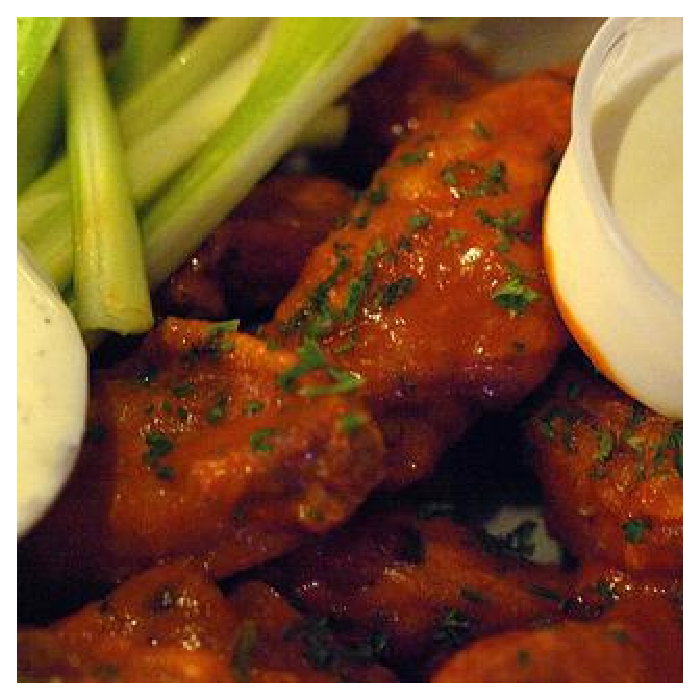
\includegraphics[width=\linewidth]{Figs4Paper/Buffalo_Wing/e1248c9ec5.eps}
%\endminipage\hfill
%\minipage{0.12\textwidth}
  %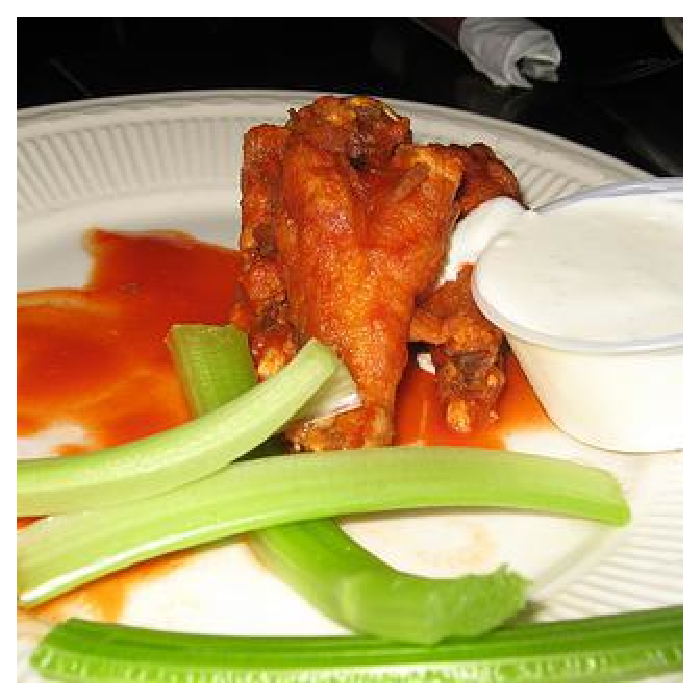
\includegraphics[width=\linewidth]{Figs4Paper/Buffalo_Wing/e1b0e74a83.eps}
%\endminipage\hfill
%\minipage{0.12\textwidth}%
  %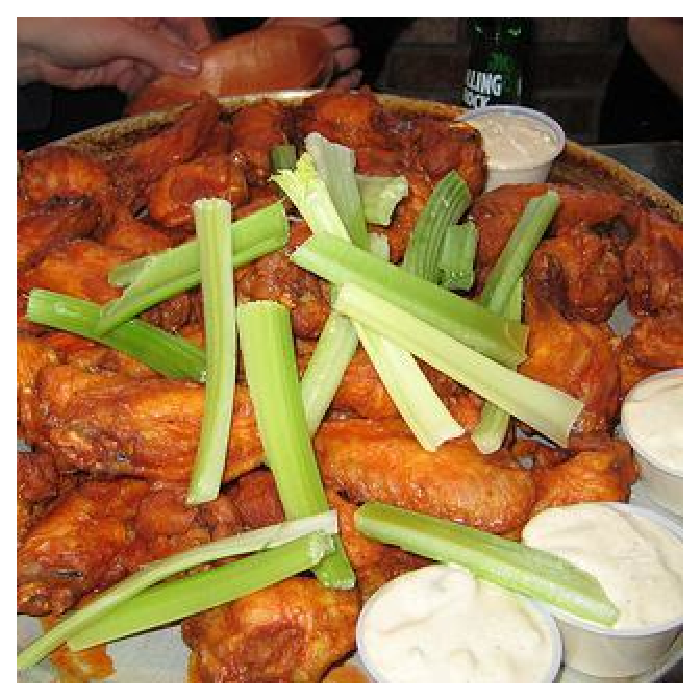
\includegraphics[width=\linewidth]{Figs4Paper/Buffalo_Wing/f192b38384.eps} 
%\endminipage
%\caption{Images of chicken wings dish with celery.}
%\label{fig:chickenwingswithcelery}
%\end{figure}

\begin{table}
\begin{center}
\begin{tabular}{|l|c|}
\hline
Food Name & Num of Images \\
\hline\hline
Clam Chowder&723\\
Jambalaya&588\\
Fish Stick&175\\
Cannelloni&230\\
Buffalo Wing&340\\
Lamb Curry&347\\
Fish And Chips&803\\
Pepperoni Pizza&773\\
Eggs Benedict&1124\\
Scotch Egg&388\\
Sashimi&818\\
Tempura&1008\\
Spaghetti&523\\
Beef Wellington&279\\
Lobster Thermidor&76\\
\hline
\end{tabular}
\end{center}
\caption{Class Label Distribution}
\label{table:classdistribution}
\end{table}

%-------------------------------------------------------------------------